% Kapitel 3 mit den entsprechenden Unterkapiteln
% Die Unterkapitel können auch in separaten Dateien stehen,
% die dann mit dem \include-Befehl eingebunden werden.
%------------------------------------------------------------------------------------
\chapter{Resultierende Softwarearchitektur}

%Dieser Abschnitt hat die Aufgabe, einen Überblick über die zu entwickelnden
%Komponenten und Subsysteme zu liefern.
\section{Komponentenspezifikation}

%In diesem Abschnitt wird die aus der Analyse der Produktfunktionen (Kapitel 2)
%resultierende Komponentenstruktur zunächst überblickartig durch ein
%Komponentendiagramm beschrieben. Die Bezeichnungen und Anzahl der Komponenten
%muss natürlich konsistent sein mit der in Kapitel 2!
Bei der Analyse der notwendigen Komponenten fallen drei Komponentenbereiche auf.
Zum einen muss der Client beachtet werden, zum anderen gibt es den Server. Der
Server besteht aus der \gls{glos:django}-App, den Templates und der Datenbank. Die App
benötigt noch die Views und den Adminbereich zur Kommunikation mit dem Client
und die Models für den Zugriff auf die Datenbank.

\begin{figure}[h]
    \begin{center}
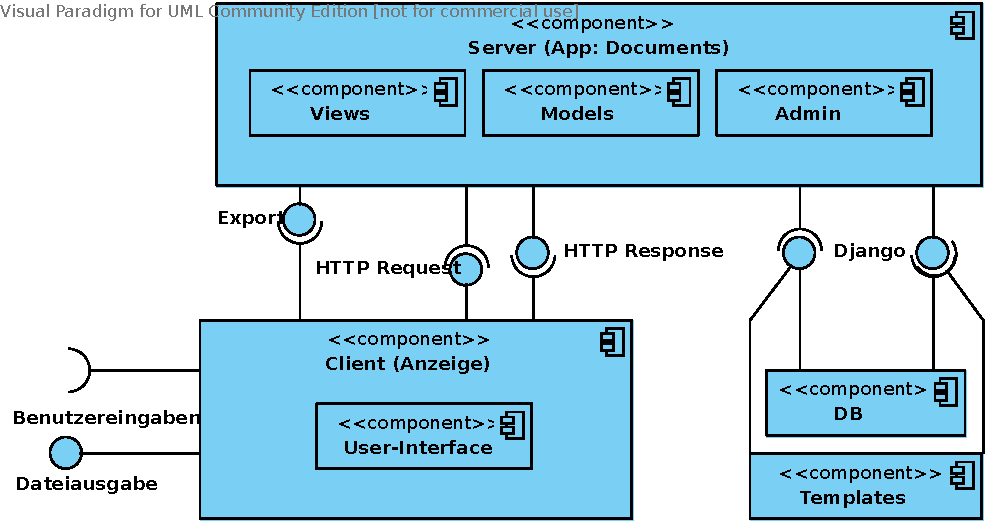
\includegraphics[width=0.8\linewidth]{bilder/Komponentendiagramm.pdf}
\caption[Komponentendiagramm]{Komponentendiagramm}
\label{Komponentendiagramm}
    \end{center}
\end{figure}

\section{Schnittstellenspezifikation}

\begin{tabular}[ht]{|l|p{0.35\linewidth}|p{0.35\linewidth}|}
\hline
Schnittstelle & \multicolumn{2}{|c|}{Aufgabenbeschreibung}\\
\hline
\hline
/S10/ HTTP Request & \multicolumn{2}{|c|}{}\\
\hline
& search(String) : List & Die Suche liefert eine Liste mit den Ergebnissen\\
& signIn(String) : boolean & Anmelden des Benutzers\\
& signOut() : boolean & Abmelden des Benutzers\\
& import(data) : boolean & Import \\
& getHistory(String) : List & liefert eine Liste der Ausgeliehen Dokumente\\
& getDoc(String) : List & liefert die Dokumentinformationen in einer Liste\\
& getView(String) : View & liefert die View, die die Aufgabenstellung erfüllt\\
\hline
/S20/Export & \multicolumn{2}{|c|}{Exportieren von Informationen}\\
\hline
& exportBibTeX() : String & Liefert einen String welcher die
Dokumentinformationen im \BibTeX -Format enthält\\
& exportAllegro() : \Gls{glos:Allegro} -kompatible Datei & Liefert eine Datei für die
\Gls{UB}\\
\hline
/S30/\gls{glos:django} & \multicolumn{2}{|c|}{Verbindung mit Datenbank}\\
\hline
& connect(String) : boolean & Verbindung zur Datenbank\\
& disconnect() : boolean & Verbindung wird beendet\\
& sendQuery(String) : List & liefert eine Liste des Ergebnisses\\
\hline
\end{tabular}





\section{Protokolle für die Benutzung der Komponenten}

In diesem Unterkapitel werden nun die Protokoll-Statecharts für alle 
Komponenten, welche in dem Komponentendiagramm \ref{Komponentendiagramm} 
vorhanden sind, dargestellt.

Für jede dieser Komponenten ist eine Wiederverwendung begrenzt sinnvoll, da alle
 diese Komponenten sehr projektspezifisch gehalten werden müssen. Sie können 
 unter Umständen in anderen Projekten eingesetzt werden, aber dann nur unter 
 größtem Anpassungsbedarf.

\subsection{Client}
\begin{figure}
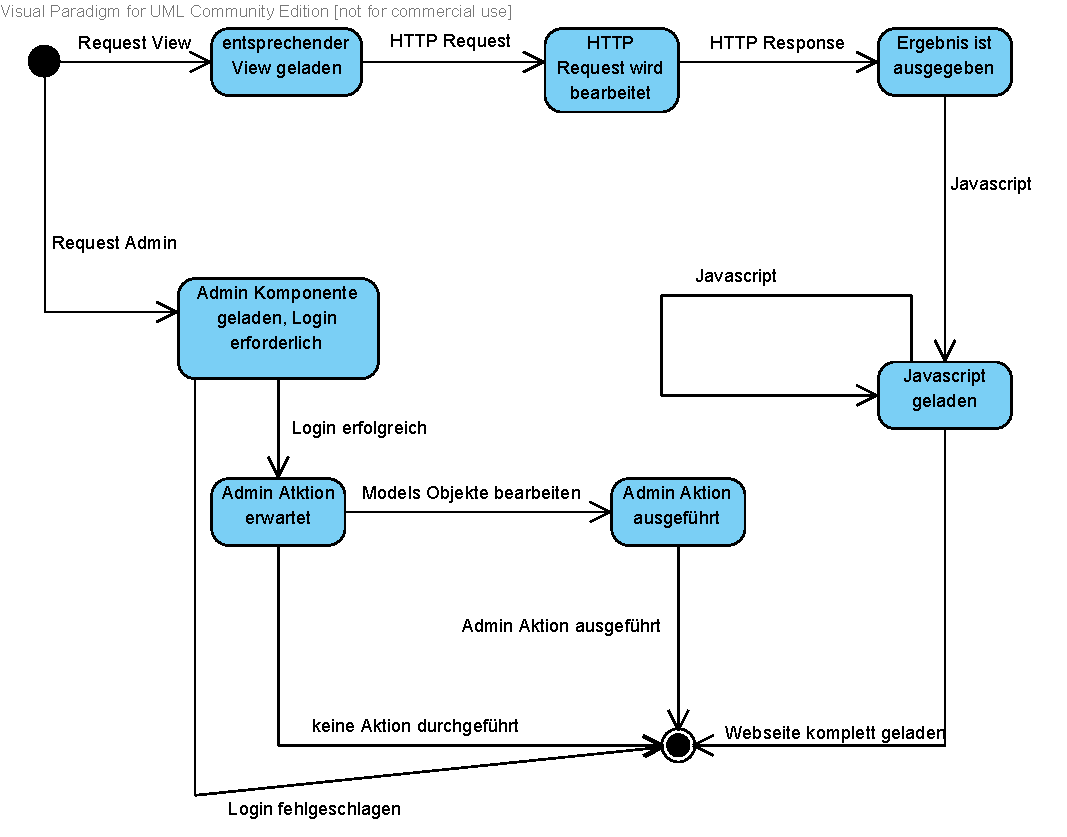
\includegraphics[width=0.8\linewidth]{bilder/KompClient.pdf}
\caption{Statechart für die Komponente Client}
\label{StClient}
\end{figure}

Vom Startzustand des Statecharts Abb.\ \ref{StClient} aus gibt es entweder die 
Möglichkeit, dass der Client eine Djangoview oder die Adminansicht aufruft. Wird 
die Adminkomponente aufgerufen, erwartet der Client zuerst eine 
Authentifizierung. Schlägt diese fehl, wird der Zugriff verweigert. Wenn sie 
aber erfolgreich ist, erwartet der Client als nächstes ein oder mehrere 
Adminaktionen oder das Beenden der Adminansicht. Ruft der Client eine Djangoview 
auf, lädt er zuerst die entsprechende View und stellt dann einen HTTP-Request. 
Sobald er das entsprechende Ergebnis erhält, gibt er es aus und lädt benötigte 
Javascripte. Damit ist die Seite komplett geladen und der Client in seinem 
Endzustand.

\subsection{View}
\begin{figure}
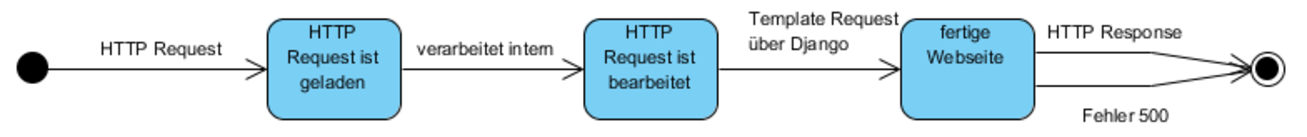
\includegraphics[width=0.8\linewidth]{bilder/KompView.pdf}
\caption{Statechart für die Komponente View}
\label{StView}
\end{figure}

Eine View (Statechart Abb.\ \ref{StView}) erhält immer zuerst einen HTTP 
Request, den sie lädt und dann verarbeitet. Ist dies geschehen, wird über das 
Djangotemplatesystem eine entsprechende fertige Webseite erzeugt und per HTTP 
Response zurückgegeben. Alternativ kann die Rückgabe auch aus einem Fehler 500 
bestehen.

\subsection{Model}
\begin{figure}
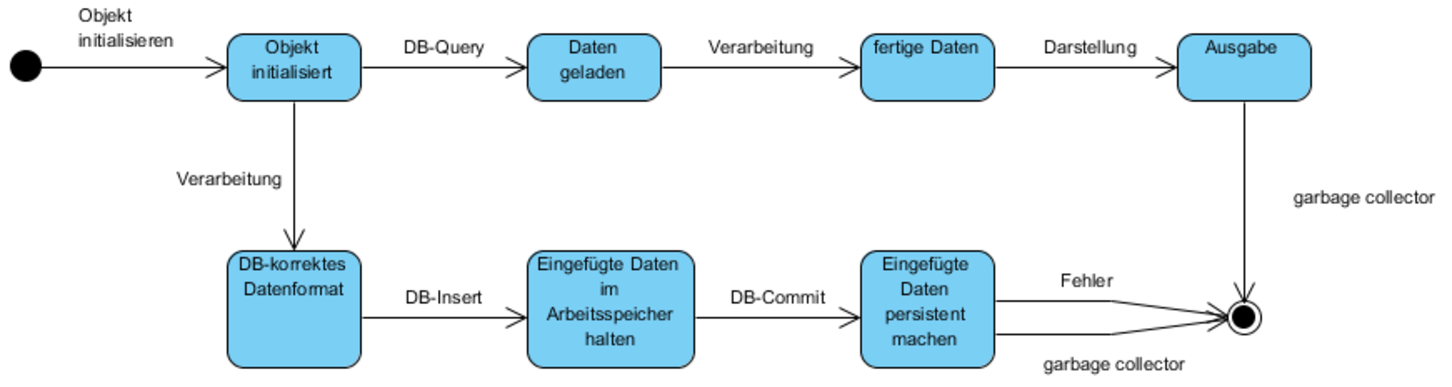
\includegraphics[width=0.8\linewidth]{bilder/KompModel.pdf}
\caption{Statechart für die Komponente Model}
\label{StModel}
\end{figure}

Nachdem das Objekt initialisiert ist, kann entweder eine Anfrage oder eine
Bearbeitung ausgeführt werden (siehe Statechart Abb.\ ref{StModel}). Wird etwas 
bearbeitet, werden die Daten zuerst in ein DB-kompatibles Format geändert. 
Nachdem DB-Insert werden die Daten noch im Arbeitsspeicher gehalten, bis der 
Commit abgeschlossen ist und die Daten konsistent gemacht wurden. Dann löscht 
der Garbage Collector das Objekt und versetzt es damit in seinen Endzustand. 
Wurde eine Anfrage gestellt, werden die Daten entsprechend der Query geladen. 
Nach der Verarbeitung der Daten und der Erstellung des Ergebnisses der Query 
wird dieses in einer Ausgabe dargestellt. Nachdem die Ausgabe beendet wurde, 
wird das Objekt vom Garbage Collector gelöscht und damit in seinen Endzustand 
versetzt.

\subsection{Admin}
\begin{figure}
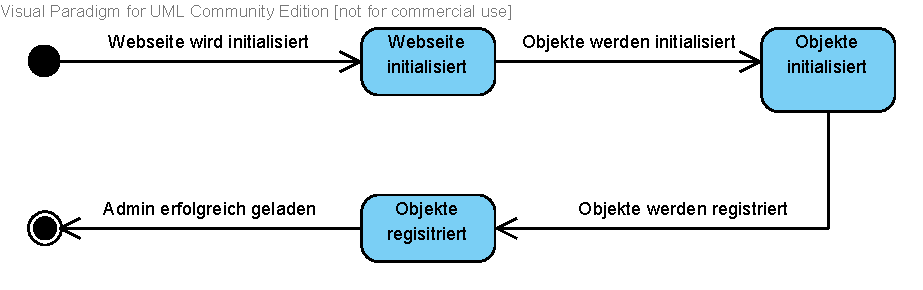
\includegraphics[width=0.8\linewidth]{bilder/KompAdmin.pdf}
\caption{Statechart für die Komponente Admin}
\label{StAdmin}
\end{figure}

Die Komponente Admin (Abb.\ \ref{StAdmin}) erstellt zuerst eine Webseite, dann 
initialisiert sie entprechende Objekte und registriert sie. Damit ist die 
Adminseite vollständig geladen. Die restliche Funktionsweise wurde bereits in 
Abb.\ \ref{StClient} beschrieben, da diese ineinander greifen.


\subsection{DB und Template}
Die Komponente \textbf{DB} wird hier nicht modelliert, da diese zunächst trivial
 ist(Anfrage an DB -> DB liefert Ergebnis) und die \textbf{DB} vollkommen durch 
 \gls{glos:django} auf die Komponente \textbf{Models} gemappt wird.

Auch auf eine Darstellung der Komponente \textbf{Template} wird verzichtet, da 
ein Template nur einen wirklichen Zustand hat, und dies ist der des Existierens. 




%In diesem Abschnitt wird mit Hilfe von Protokoll-Statecharts die korrekte
%Verwendung der zu entwickelnden Komponenten dokumentiert. Dies ist insbesondere
%für diejenigen Komponenten notwendig, für die eine Wiederverwendung möglich
%erscheint oder sogar bereits geplant ist.

%Begründen Sie für welche Komponenten eine Wiederverwendung sinnvoll erscheint
%und für welche nicht!

%Fügen Sie so viele Statechartdiagramme ein, wie sie Komponenten gefunden haben.
